\chapter*{Dodatak: Prikaz aktivnosti grupe}
		\addcontentsline{toc}{chapter}{Dodatak: Prikaz aktivnosti grupe}
		
		\section*{Dnevnik sastajanja}
		
		\textbf{\textit{Kontinuirano osvježavanje}}\\
		
		 \textit{U ovom dijelu potrebno je redovito osvježavati dnevnik sastajanja prema predlošku.}
		
		\begin{packed_enum}
			\item  Uvodni sastanak
			
			\item[] \begin{packed_item}
				\item Datum: 19. listopada 2023.
				\item Prisustvovali: A.Hohnjec, M.Pavić, A.Kantarević, L.Ivčević, B.Zrakić, F.Vrbić, A.Zglavnik
				\item Teme sastanka:
				\begin{packed_item}
					\item  Upoznavanje sudionika projektnog tima
				\end{packed_item}
			\end{packed_item}
			
			\item  Sastanak o raspodjeli poslova
			
			\item[] \begin{packed_item}
				\item Datum: 25. listopada 2023.
				\item Prisustvovali: A.Hohnjec, M.Pavić, A.Kantarević, L.Ivčević, B.Zrakić, F.Vrbić, A.Zglavnik
				\item Teme sastanka:
				\begin{packed_item}
					\item  Dogovor o raspodjeli poslova pri izradi aplikacije
					\item  Dogovor o raspodjeli poslova pri izradi dokumentacije
					\item  Dogovor o načinu izvršavanja projekta
				\end{packed_item}
			\end{packed_item}
			
			\item  Merganje pojedino izrađene dokumentacije
			
			\item[] \begin{packed_item}
				\item Datum: 30. listopada 2023.
				\item Prisustvovali: A.Hohnjec, M.Pavić, A.Kantarević, L.Ivčević, B.Zrakić, F.Vrbić, A.Zglavnik
				\item Teme sastanka:
				\begin{packed_item}
					\item  Merganje pojedino izrađene dokumentacije
				\end{packed_item}
			\end{packed_item}
			
				\item  Dogovor za daljnji napredak aplikacije
			
			\item[] \begin{packed_item}
				\item Datum: 15. prosinca 2023.
				\item Prisustvovali: A.Hohnjec, M.Pavić, A.Kantarević, L.Ivčević, B.Zrakić, F.Vrbić, A.Zglavnik
				\item Teme sastanka:
				\begin{packed_item}
					\item  Raspodjela daljnjih poslova
					\item  Pregled dosad napravljenoga
					\item  Dogovor za rad kroz praznike
				\end{packed_item}
			\end{packed_item}
			
				\item  Pregled napravljenog kroz praznike
			
			\item[] \begin{packed_item}
				\item Datum: 4. siječnja 2024.
				\item Prisustvovali: A.Hohnjec, M.Pavić, A.Kantarević, L.Ivčević, B.Zrakić, F.Vrbić, A.Zglavnik
				\item Teme sastanka:
				\begin{packed_item}
					\item  Pregled napravljenog programskog dijela
					\item  Davanje dodatnih informacija za izradu dokumentacije
				\end{packed_item}
			\end{packed_item}
			
				\item  Dogovor oko završnih detalja
			
			\item[] \begin{packed_item}
				\item Datum: 15. siječnja 2024.
				\item Prisustvovali: A.Hohnjec, M.Pavić, A.Kantarević, L.Ivčević, B.Zrakić, F.Vrbić, A.Zglavnik
				\item Teme sastanka:
				\begin{packed_item}
					\item  Završni detalji pri izradi aplikacije
					\item  Završavanje sa izradom dokumentacije
				\end{packed_item}
			\end{packed_item}
			%
			
		\end{packed_enum}
		
		\eject
		\section*{Tablica aktivnosti}
		
			\textbf{\textit{Kontinuirano osvježavanje}}\\
			
			 \textit{Napomena: Doprinose u aktivnostima treba navesti u satima po članovima grupe po aktivnosti.}

			\begin{longtblr}[
					label=none,
				]{
					vlines,hlines,
					width = \textwidth,
					colspec={X[7, l]X[1, c]X[1, c]X[1, c]X[1, c]X[1, c]X[1, c]X[1, c]}, 
					vline{1} = {1}{text=\clap{}},
					hline{1} = {1}{text=\clap{}},
					rowhead = 1,
				} 
			
				\SetCell[c=1]{c}{} & \SetCell[c=1]{c}{\rotatebox{90}{\textbf{Antonio Hohnjec}}} & \SetCell[c=1]{c}{\rotatebox{90}{\textbf{Marko Pavić }}} &	\SetCell[c=1]{c}{\rotatebox{90}{\textbf{Armis Kantarević }}} & \SetCell[c=1]{c}{\rotatebox{90}{\textbf{Luka Ivčević }}} &	\SetCell[c=1]{c}{\rotatebox{90}{\textbf{Benjamin Zrakić }}} & \SetCell[c=1]{c}{\rotatebox{90}{\textbf{Filip Vrbić }}} &	\SetCell[c=1]{c}{\rotatebox{90}{\textbf{Antonio Zglavnik }}} \\  
				Upravljanje projektom 		&10  &  &  &  &  &  & \\ 
				Opis projektnog zadatka 	&2  &  &  &  &  &  & \\ 
				
				Funkcionalni zahtjevi       &  &  &  &  &  &  &  \\ 
				Opis pojedinih obrazaca 	&  &  &  &1  &1  &1  &  \\ 
				Dijagram obrazaca 			&  &  &  &  &3  &2  &  \\ 
				Sekvencijski dijagrami 		&  &  &  &2  &  &  &  \\ 
				Opis ostalih zahtjeva 		&  &  &1  &  &  &  &  \\ 

				Arhitektura i dizajn sustava	 &  &1  &  &  &  &  &  \\ 
				Baza podataka				&  &4  &3  &  &  &  &   \\ 
				Dijagram razreda 			&  &  &  &  &  &  & 2  \\ 
				Dijagram stanja				&  &  &  &  &  &1  &  \\ 
				Dijagram aktivnosti 		&  &  &  &1  &  &  &  \\ 
				Dijagram komponenti			&  &  &  &  &1  &  &  \\ 
				Korištene tehnologije i alati 		&  &  &1  &  &  &  &  \\ 
				Ispitivanje programskog rješenja 	&3  &  &  &  &  &  &  \\ 
				Dijagram razmještaja			&  &  &  &  &2  &  &  \\ 
				Upute za puštanje u pogon 		&1  &  &  &  &  &  &  \\  
				Dnevnik sastajanja 			&1  &  &  &  &  &  &  \\ 
				Zaključak i budući rad 		&1  &  &  &  &  &  &  \\  
				Popis literature 			&1  &  &  &  &  &  &  \\  
				&  &  &  &  &  &  &  \\ \hline 
				\textit{Dodatne stavke kako ste podijelili izradu aplikacije} 			&  &  &  &  &  &  &  \\ 
				\textit{npr. izrada početne stranice} 				&  &1  &  &  &1  &  &1  \\  
				\textit{izrada baze podataka} 		 			&  &  &1  &1  &  &1  & \\  
				\textit{spajanje s bazom podataka} 							&1  &  &  &  &  &  &  \\ 
				\textit{deployment} 							&1  &  &  &  &  &  &  \\  
				 							&  &  &  &  &  &  &\\ 
			\end{longtblr}
					
					
		\eject
		\section*{Dijagrami pregleda promjena}
		
		\begin{figure}[H]
			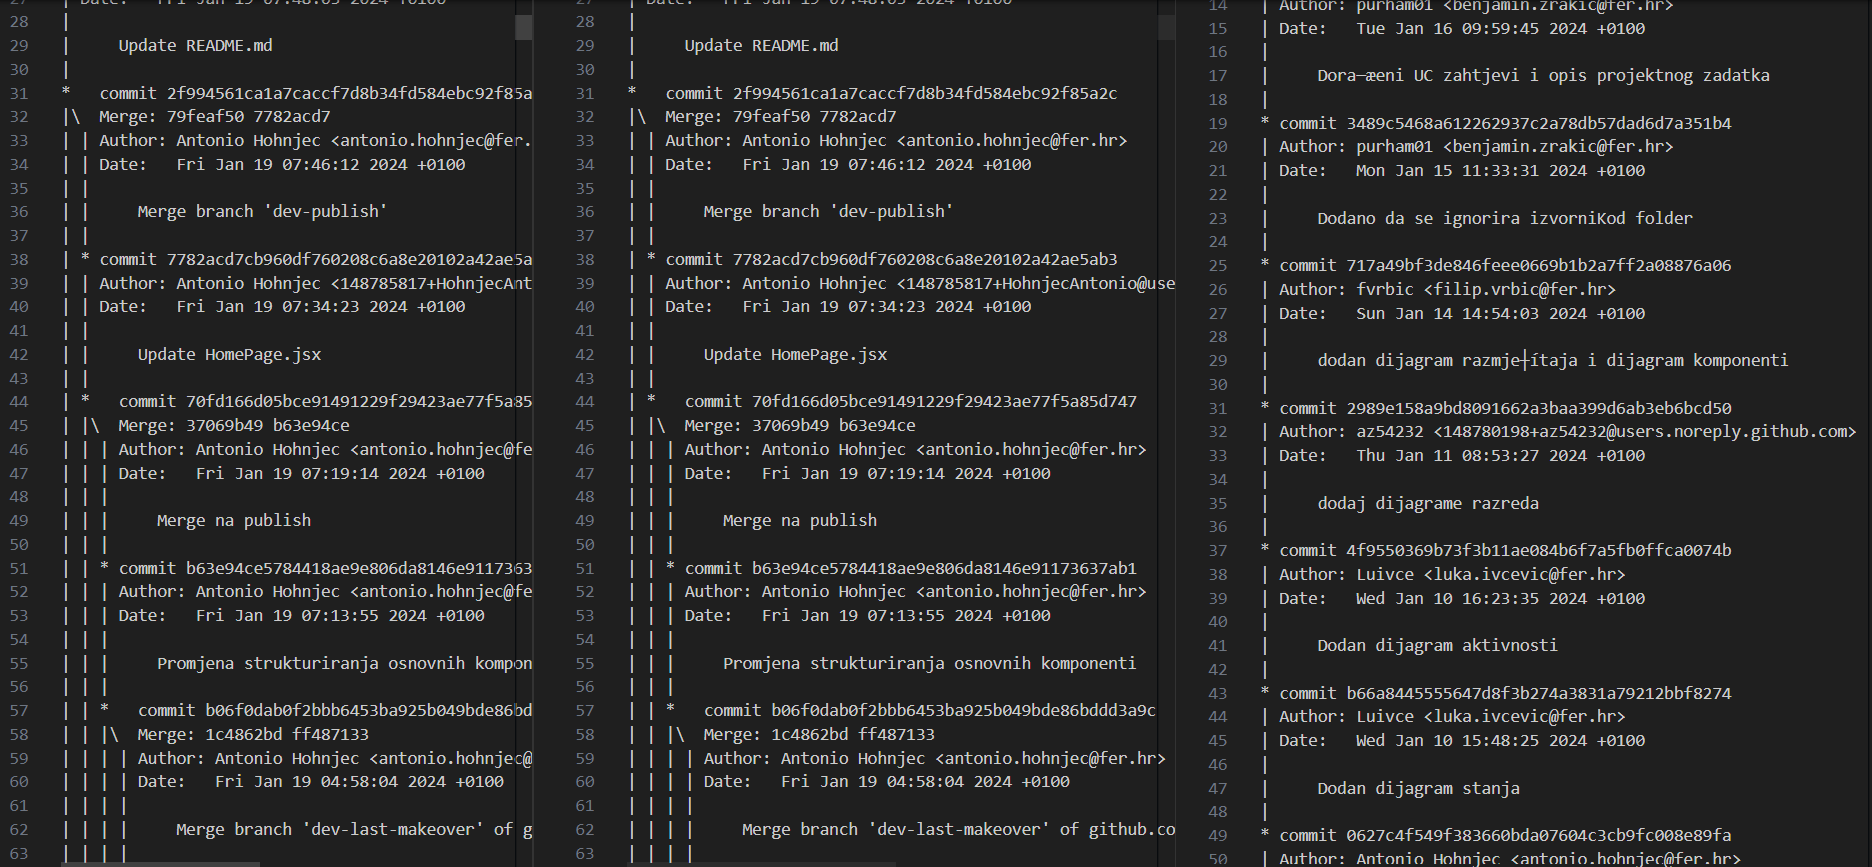
\includegraphics[scale= 0.45]{slike/Logs.png}
			\centering
			\caption{Github logs master, publish i dokumentacija grana}
			\label{fig:Github logs}
		\end{figure} 
	